\documentclass[18pt]{article}
\usepackage{amsmath,amsfonts,amssymb}
\usepackage{natbib}
\usepackage{booktabs}
\usepackage[utf8]{inputenc}
\usepackage[T1]{fontenc}
\usepackage{amssymb}
\usepackage[version=4]{mhchem}
\usepackage{stmaryrd}
\usepackage{bbold}
\usepackage{nopageno}
\usepackage{hyperref}
\usepackage{bookmark}
\usepackage{mathtools}
\usepackage{pdfpages}
\usepackage{geometry}
\author{Adam Handwerger}
\pagestyle{plain}
\NewDocumentCommand{\angled}{me{^_}}{%
  \langle #1\rangle
  ^{\smash[t]{\mathstrut}\IfValueT{#2}{#2}}% superscript
  _{\smash[b]{\mathstrut}\IfValueT{#3}{\!#3}}% subscript
}
\DeclareMathAlphabet{\bbold}{U}{bbold}{m}{n}
\newcommand{\id}{\ensuremath{\bbold{1}}}
\begin{document}
\begin{flushleft}
Exercise 1\\
Let V be a subspace of dimension d of a Hilbert space H. Show that the \\
projection of $x \in \mathbb{R}^p$ onto V can be written as\\
\vspace{.4cm}
$\hspace{3cm} \pi_V(x)=\sum\limits_{i=1}^d \langle x_i,v_i \rangle v_i$\\
\vspace{.4cm}
where $v_i$ form an orthonormal basis, B for V.\\
\vspace{.4cm}
The following properties hold for V:\\
1. If $x\in V,\pi_V(x)=x$\\
2. For any $v\in V,x \in \mathbb{R}^p, \langle x-\pi_V(x),v\rangle=0$\\
\vspace{.4cm}
Proof: Let $v_i$ be a orthonomal basis, B for V. Since $\pi_V(x)\in V, \pi_V(x)$ can be written as\\
$\hspace{3cm} \pi_V(x)=\sum\limits_i \alpha_i v_i$\\
for $\alpha_i \in \mathbb{R}$.
\vspace{.4cm}
Then by property 2 and for any element $v_j \in B$ we have\\
\vspace{.4cm}
$\langle x-\sum\limits_i \alpha_i v_i,v_j \rangle=0 \implies$\\
$\langle x,v_j \rangle=\langle \sum_i \alpha_i v_i,v_j\rangle=\sum_i \alpha_i \langle v_i,v_j \rangle=\sum_i \alpha_i \delta_{ij}=\alpha_j$\\
\vspace{.4cm}
Thus $\alpha_j=\langle x,v_j \rangle$ and $\pi_V(x)=\sum\limits_i \alpha_i v_i=\sum\limits_i \langle x,v_j \rangle v_j$\\
\vspace{.4cm}
Exercise 3
$$
R(x)=\dfrac {x M x'}{x^{\top} x}
$$

\vspace{.4cm}
Show that R(x) is maximized when it equals the largest eigenvalue of M. This\\
occurs when x is the associated eigenvector.\\
\vspace{.4cm}
Let $M=P \Lambda P^{\top}$ be the spectral decompostion of M. The columns of P are the \\
eigenvectors of M and form an orthonormal basis, B of dimension d. The dimension d is equal to the number of eigenvectors with non-zero
eigenvectors. We may complete B by argumenting it by (p-d) additional vectors that are orthonoral to each other and to B. Likewise, we also extend $\Lambda$ as\\
$$
\Gamma=
\begin{bmatrix}
   \lambda_1 & & & & &\huge0\\ 
   &  &  \ddots & & & \\
   &  &  & \lambda_d & &  \\
   &  &  &  & 0 & \\
   &  &  &  & & & \ddots &\\
   &\huge0  &  &  &  & & & 0
\end{bmatrix}
$$

\vspace{.4cm}
Then M can be written
$$
M=Q  \Gamma Q^{\top}
$$
with $QQ^{\top}=I$ and $Q^{\top}Q=I$.
\vspace{.4cm}
Defining $y=Q^{\top}x$, R(x) can be written
\vspace{.4cm}
$R(x)=\dfrac{y^{\top}\Gamma y}{y^{\top}y}=\dfrac{\sum\limits_{i=1}^p \lambda_i y_i^2}{\sum\limits_{j=1}^p y_j}=\sum\limits_{i=1} \lambda_i \left(\dfrac{ y_i^2}{\sum\limits_{j=1}^p y_j}\right)$\\
\vspace{.4cm}
If we set $w_i$=$\frac{ y_i^2}{\sum\limits_{j=1}^p y_j^2}$ then $\sum_i w_i=1$ and R(x) can be seen to be a\\
convex combination of the eigenvalues of M. This implies that $R(x)$ will reach a maximum when $R(x)=\lambda_{\max}$, and all the terms in the sum are zero except for this one.
If this index is the jth then $w_{\max}=\mathbb{1}_j$. If we order the eigenvalues $\{v_1,...v_d\}$ from largest to smallest, then $\max_{x\in\mathbb{R}^p} R(x)=\lambda_1$ and argmax $R(x)=v_1$.\\
\vspace{.4cm}
Excercise 6\\
\vspace{.4cm}
The centered kernel is given by\\
\vspace{.4cm}
$\tilde{K}(x,y)=\left\langle K(\cdot,x)-\frac{1}{n}\sum_i K(\cdot,x_i), K(\cdot,y)-\frac{1}{n}\sum_i K(\cdot,x_i)\right\rangle=$\\
$\langle \frac{1}{n}\sum_i\left(K(\cdot,x)- K(\cdot,x_i)\right), \frac{1}{n}\sum_i\left(K(\cdot,y)- K(\cdot,x_i)\right)\rangle$\\
\vspace{.4cm}
Show that is symmetric and p.d.\\
\vspace{.4cm}
$\tilde{K}(x,y)=\tilde{K}(y,x)$ follows because the inner product is symmetric.\\
\vspace{.4cm}
Positive definiteness follows from the following:\\
\vspace{.4cm}
$\sum\limits_{kl} \alpha_k \alpha_l \tilde{K}(x_k,x_l)=\left\langle \frac{1}{n}\sum\limits_i\left(\sum\limits_k \alpha_k K(\cdot,x)- K(\cdot,x_i)\right), \frac{1}{n}\sum\limits_i\left(\sum\limits_l \alpha_l K(\cdot,y)- K(\cdot,x_i)\right)\right\rangle=$\\
$\parallel \frac{1}{n}\sum\limits_{i} \sum\limits_{k} \alpha_k \left(K(\cdot,x_k)-K(\cdot,x_i)\right) \parallel^2=\parallel \sum\limits_{k} \alpha_k \left( K(\cdot,x_k)-\frac{1}{n}\sum\limits_{i} K(\cdot,x_i)\right) \parallel^2 \geq0$\\
\vspace{.4cm}
Exercise 7\\
\vspace{.4cm}
Show that that the RKHS of $\tilde{K}$ is given by the following:\\
\vspace{.4cm}
$\tilde{H}=\left\{f_g(\cdot)=g(\cdot)-\frac{1}{n}\sum\limits_i g(x_i),\text{ }g\in H \right\}$\\
\vspace{.4cm}
with $\langle f_{g_1},f_{g_2}\rangle=\langle g_1,g_2\rangle$\\
\vspace{.4cm}
We see that $\tilde{K}=f_K \in \tilde{H}$ since H is a vector space which implies\\
\vspace{.4cm}
$K(\cdot,x)-\frac{1}{n} \sum\limits_i K(\cdot,x_i) \in H$\\
Also $\tilde{K}$ has the reproducing property since\\
\vspace{.4cm}
$\langle \tilde{K}(\cdot,x),f_g \rangle_{\tilde{H}}= \langle f_{K(\cdot,x)},f_g \rangle_{\tilde{H}}=$\\
$\langle K(\cdot,x),\frac{1}{n}\sum\limits_i(g(\cdot)-g(x_i))\rangle_H=\frac{1}{n}\sum\limits_i (g(x)-g(x_i))=$\\
$g(x)-\frac{1}{n} \sum\limits_i g(x_i)=f_g(x)$\\
\vspace{.4cm}
The second line follows from the reproducing property of H.\\
\vspace{.4cm}
Exercise 8\\
\vspace{.4cm}
Show that for any $f\in \tilde{H}, \sum\limits_i^n f(x_i)=0$\\
\vspace{.4cm}
Proof: $f_g \in \tilde{H} \implies g\in H$. Therefore,\\
\vspace{.4cm}
$\frac{1}{n} \sum\limits_i^n f(x_i)=\frac{1}{n} \sum\limits_i^n g(x_i)-\frac{1}{n^2}\sum\limits_{ij} g(x_j)=$\\
$\frac{1}{n} \sum\limits_i^n g(x_i)-\frac{n}{n^2}\sum\limits_j g(x_j)=0$\\
\vspace{.4cm}
Exercise 9\\
\vspace{.4cm}
Defining $w_j=\Lambda^{\frac{1}{2}} P^{\top} \alpha_j$. Show that in PCA, the optimization problem can be\\
written as\\
\vspace{.4cm}
$\hspace{2cm}$ maximize $\sum\limits_{j=1}^d w_j^{\top} \Lambda w_j \text{ with } w_i^{\top}w_j=\delta_{ij}$\\
\vspace{.4cm}
Since $w_j^{\top}=(\Lambda^{\frac{1}{2}} P^{\top} \alpha_j)^{\top}=\alpha_j^{\top} P \Lambda^{\frac{1}{2}}$ and $PP^{\top}=I$ we have\\
\vspace{.4cm}
$K=P^{\top} \Lambda P \implies K^2=(P^{\top} \Lambda P)(P^{\top} \Lambda P)=(P^{\top}\Lambda^{\frac{1}{2}}) \Lambda (\Lambda^{\frac{1}{2}} P)\implies$\\
\vspace{.4cm}
$\sum\limits_j \alpha_j K^2 \alpha_j=\sum\limits_j w_j^{\top} \Lambda w_j$\\
Also $\alpha_j^{\top}K\alpha_k=\alpha_j^{\top}K\alpha_k=\alpha_j^{\top} P^{\top} \Lambda^{\frac{1}{2}}\Lambda^{\frac{1}{2}} P \alpha_k =\delta_{jk} \implies$\\
$w_j^{\top}w =\delta_{jk}$ is the contraint in terms of w.\\
\vspace{.4cm}
Thus as suggested above, the PCA optimization problem can be reframed in terms of the variable w.\\
\vspace{.4cm}
Exercise 10\\
Use the procedure in exercise 3 to show that the solution to the kernelized PCA is $w_{\mathbb{1}}$.\\
\vspace{.4cm}
Let $\Gamma=\text{diag}(\lambda_1,\dots,\lambda_d,0,\dots,0)$ where $\lambda_1 \leq \lambda_2 \leq \dots \leq 0$
In this case $Q=P$ and $M=I \Gamma I$ and $y=Qw=Iw=w \implies$ \\
\vspace{.4cm}
$\hspace{3cm} R(x)=\sum\limits_{i=1}^p \lambda_i\dfrac{ y_i^2}{\sum\limits_{j=1}^p y_j^2}\equiv \sum\limits_{i=1}^p \lambda_i z_i$\\
\vspace{.4cm}
Once again for $R(x)$ is a convex combination combination of the eigenvalues of M. This implies that $R(x)$ will reach a maximum when $R(x)=\lambda_{\max}$, so all the terms in the sum are zero except\\
for, say the jth so $y_{\max}=Iw_{\max}=\large{\mathbb{1}}_j$. The PCA algorithm aims maximize all $R(x)$ over a set of points $\{x_1...x_d\}$ where each point $x_i \in \mathbb{R}^d$. This is equivalent to finding the points that maximize\\
the sum\\
\vspace{.4cm}
$\hspace{2cm} S= \text{maximize } \sum\limits_{i=1}^d x_i^{\top}Mx_i \text{  such that }\langle x_i,x_j \rangle=\delta_{ij}$\\
\vspace{.4cm}
From the discussion above, we know that the solution is set the normalized\\
eigenvectors $\{v_1,v_2,...v_d\}$ of K, ordered from largest to smallest by eigenvalue.\\
\vspace{.4cm}


2 Kernel centering\\
\vspace{.4cm}
Let $\mathcal{X}=\mathbb{R}^d$. Show that for $K(x,y)=x^{\top}y$ the centered kernel is given by\\
$$
\tilde{K}(x,y)=(x-\bar{x})^{\top}(y-\bar{x}) \bar{x}
$$
with
$$\bar{x}=\dfrac{1}{n}\sum\limits_{i=1}^n x_i
$$
\vspace{.4cm}
$\tilde{K}(x,y)=\left\langle K(\cdot,x)-\frac{1}{n}\sum_i K(\cdot,x_i), K(\cdot,y)-\frac{1}{n}\sum_i K(\cdot,x_i)\right\rangle=$\\
$\langle K(\cdot,x),K(\cdot,y)\rangle-\frac{1}{n}\sum\limits_i \langle K(\cdot,x_i),K(\cdot,y) \rangle-\frac{1}{n}\sum\limits_i \langle K(\cdot,x_i),K(\cdot,x) \rangle+$\\
$\frac{1}{n^2}\sum\limits_{ij} \langle K(\cdot,x_i),K(\cdot,x_j) \rangle=$\\
$x^{\top}y+\dfrac{y}{n} \sum\limits_i \bar{x_i}^{\top}-\dfrac{x}{n} \sum\limits_i \bar{x_i}^{\top}+\left( \dfrac{1}{n} \sum\limits_i \bar{x_i}^{\top}\right)\left(\dfrac{1}{n} \sum\limits_j \bar{x_j}\right)=$\\
$x^{\top}y-\bar{x}^{\top}y-\bar{x}^{\top}x+\bar{x}^{\top}\bar{x}=(x^{\top}-\bar{x}^{\top})(y-\bar{x})=(x-\bar{x})^{\top}(y-\bar{x})$\\
\vspace{.4cm}
3. Coding\\
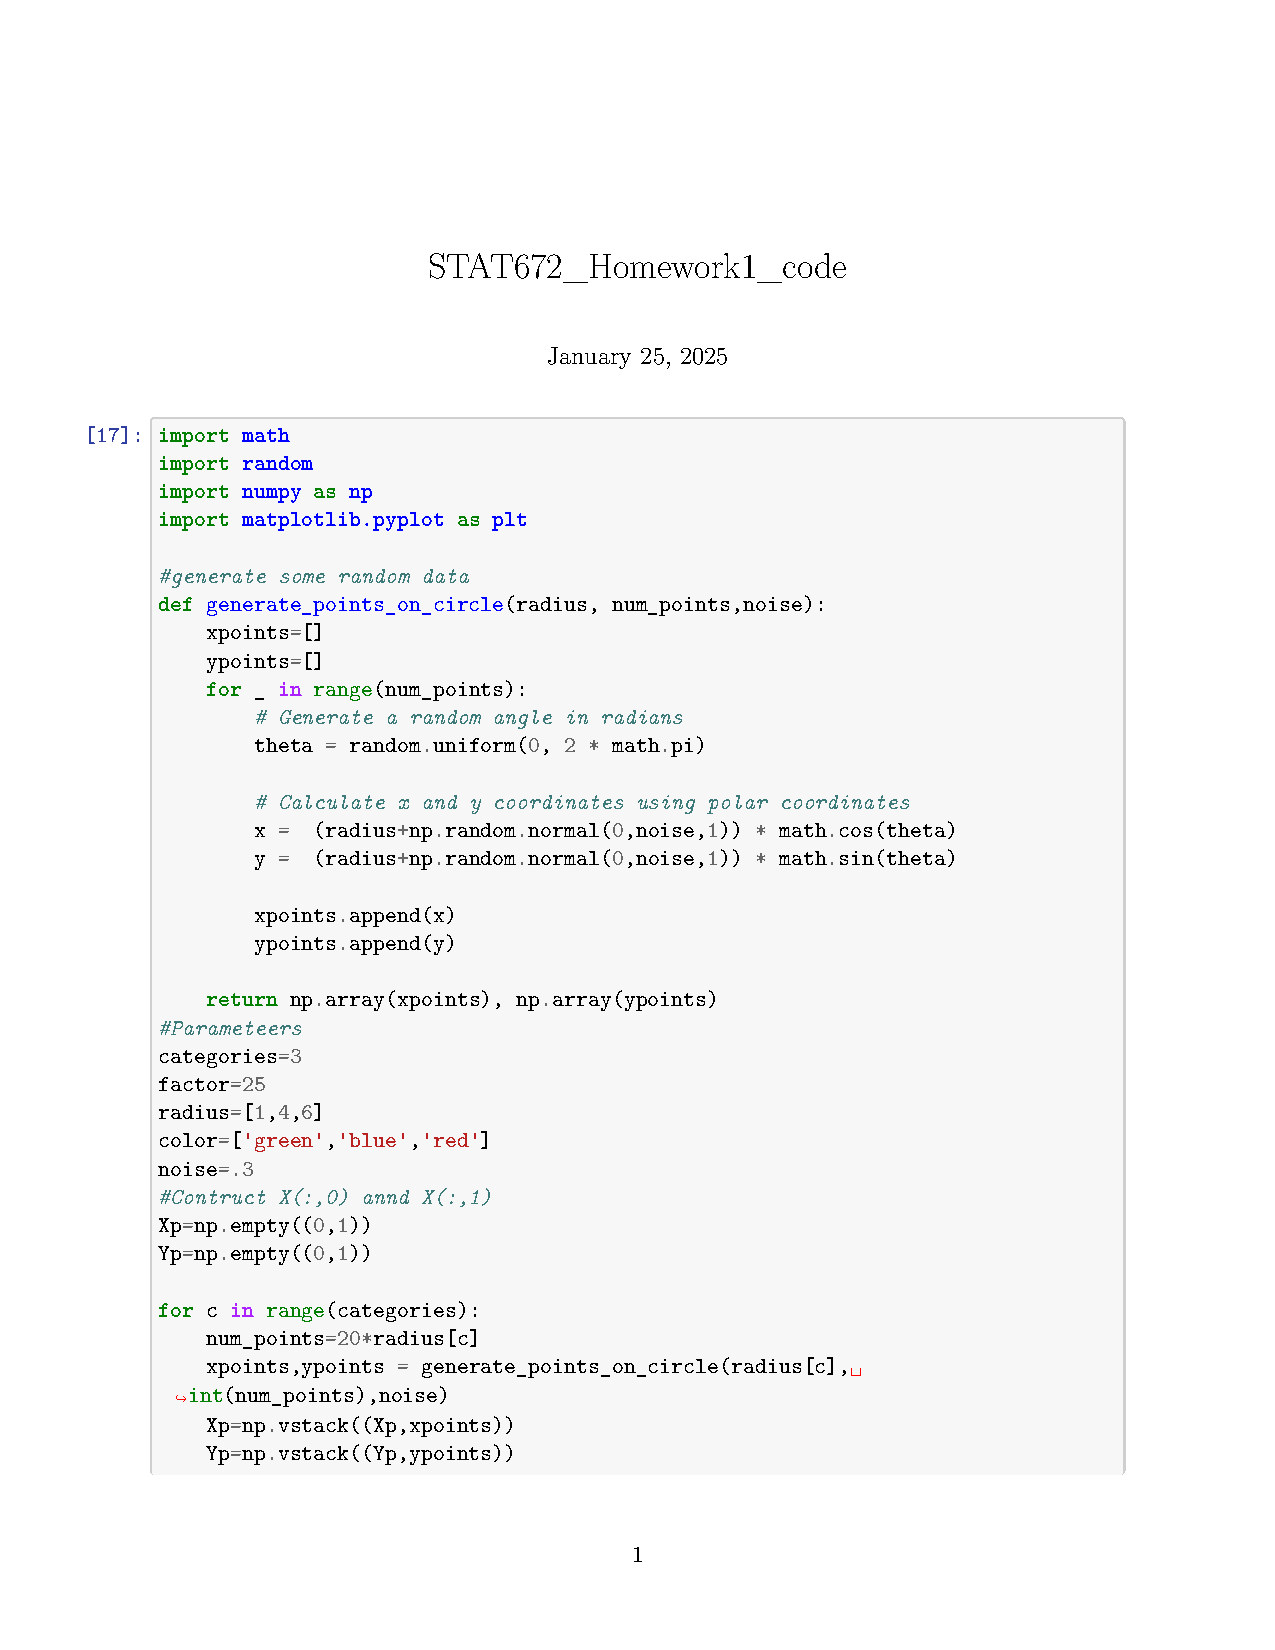
\includepdf[pages=-]{STAT672Homework1_code.pdf}

Bonus\\
\vspace{.4cm}
1. Yes, the PCA and KPCA reutrn the same results if KPCA uses a linear kernel. See plots below.\\
\vspace{.4cm}
2. Let V be of maximaal dimension d and compare the complexity of each algorithm.
\vspace{.4cm}
The PCA is an optimization problem with cost function\\
$\sum\limits_{j=1}^d v_j (\frac{1}{n} \sum\limits_{i=1}^n x_i x_i^{\top}) v_j$, whereas the optimation problem for KPCA uses\\
$\frac{1}{n}\sum\limits_{j=1}^d \alpha_j^{\top} K^2 \alpha_j$.\\
\vspace{.4cm}
Upon comparison of the two cost functions the difference in complexity is mainly given by the difference between
calculating $\sum\limits_{i=1}^n x_i x_i^{\top}$ vs. calculating $K^2$. Let's analyse the number of operation for each.
$x_i$ has d rows so $x_i x_i^{\top}$ requires $d \times d$ products and the sum over n of them requires $n\times d^2$ products.
For each entry in $K^2$ there are n products and n summations. Since there are $n^2$ matrix entries there are $n^3$ products and $n^3$ summations.\\
\vspace{.4cm}
Since products are much more compuational expensive the difference between thee two algoithms is between the calaculation of $n \times d^2$ and $n^3$ products.Since d is general is less than n, PCA will \\
generally be faster than KPCA for a linear kernel. Only when the dimension of V is large compared with the number of samples would KPCA be, in thiss case, a better choice.\\
Using the data problem 3 with 275 samples with d=2, the elapsed time for PCA was .78 ms and for KPCA .81 ms.\\
\newgeometry{top=5cm}
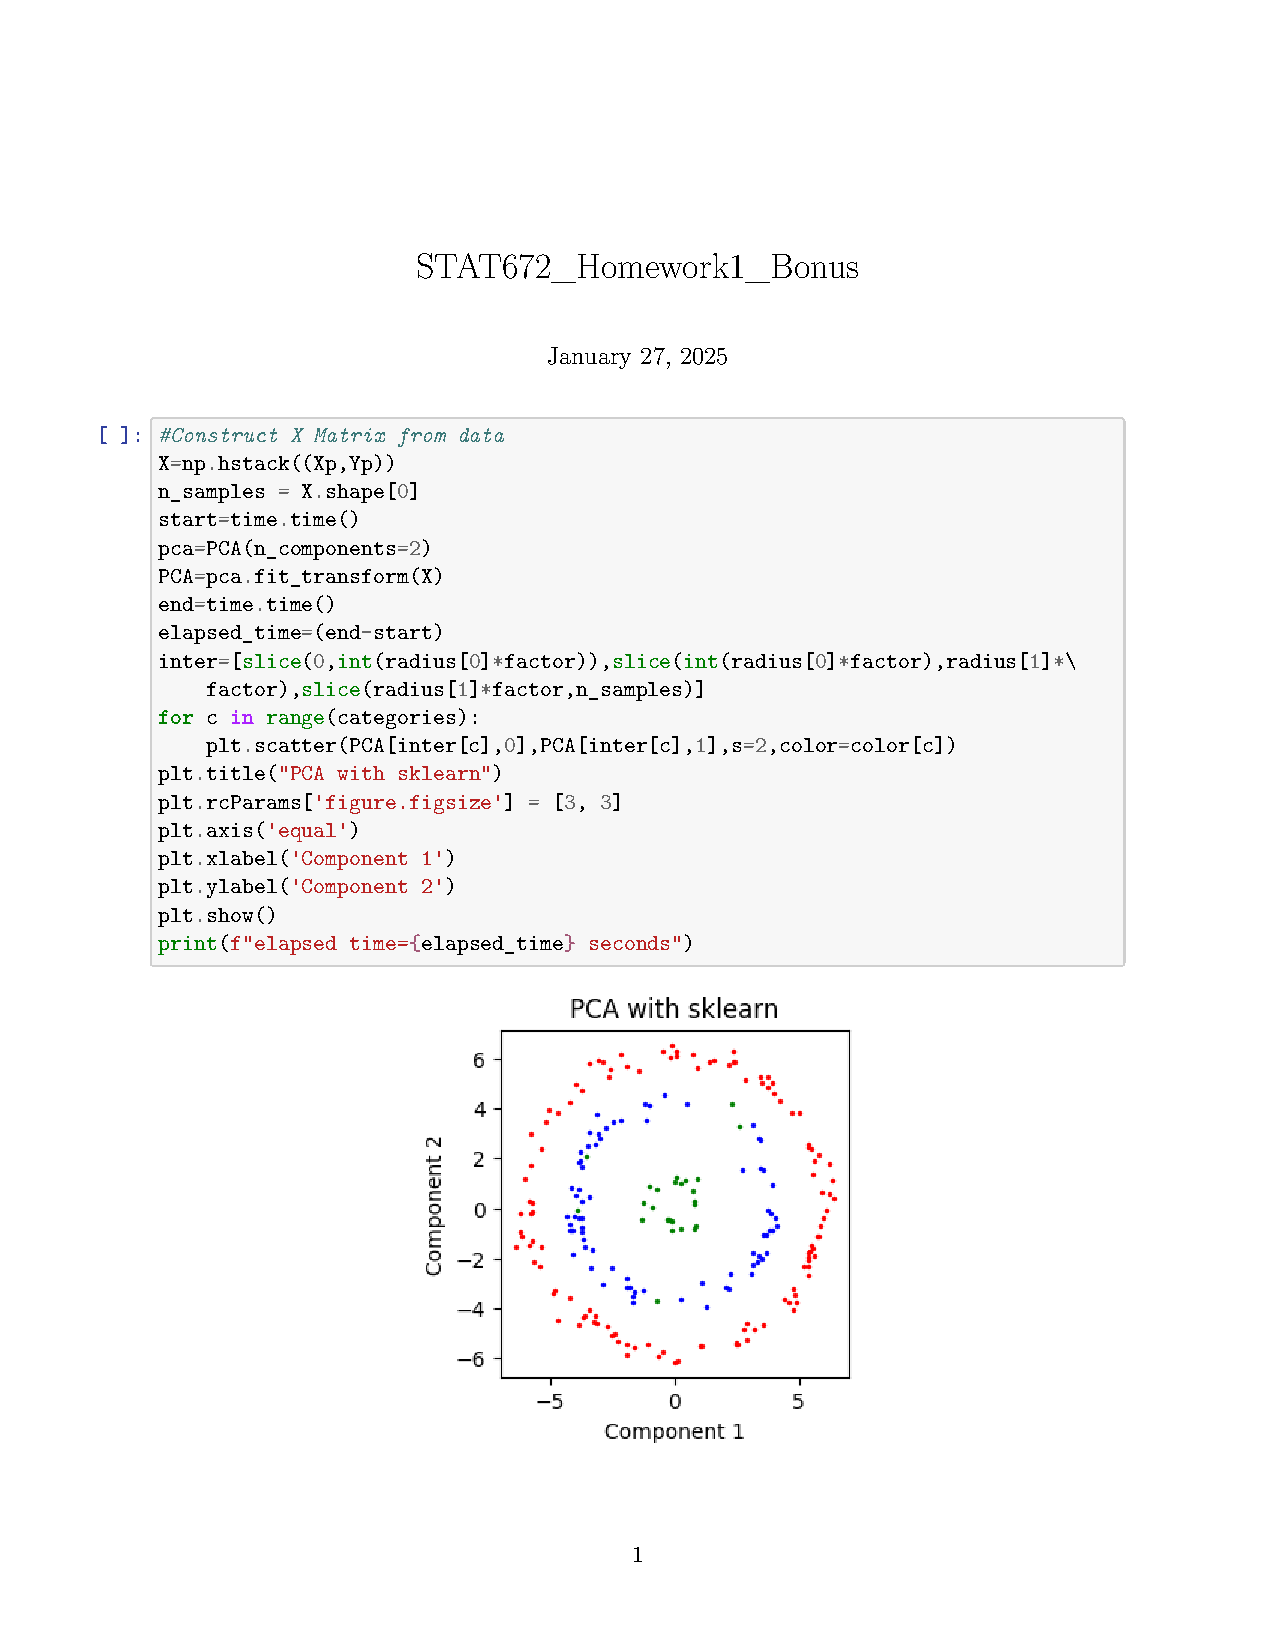
\includepdf[pages=-]{STAT672_Homework1_Bonus.pdf}

\end{flushleft}
\end{document}
    













